\documentclass[aspectratio=169]{beamer}
\setbeamertemplate{navigation symbols}{}
\usepackage{color,amsmath,comment, subfigure}
\usepackage{booktabs}



%%%%%%%%%%%%%%%%%%%%%%%%%%
\title[]{Lecture 19: Social media and society}
\author[]{Matthew J. Salganik}
\institute[]{Sociology 204: Social Networks\\Princeton University}
\date[]{
2/2 Facebook NewsFeed and political polarization
\vfill

\begin{flushleft}
\vspace{0.6in}

\includegraphics[width=0.1\textwidth]{figures/cc.png}
\end{flushleft}
}

\begin{document}
%%%%%%%%%%%%%%%%%%%%%%%%%%%
\frame{\titlepage}
%%%%%%%%%%%%%%%%%%%%%%%%%%%
\begin{frame}

\begin{center}
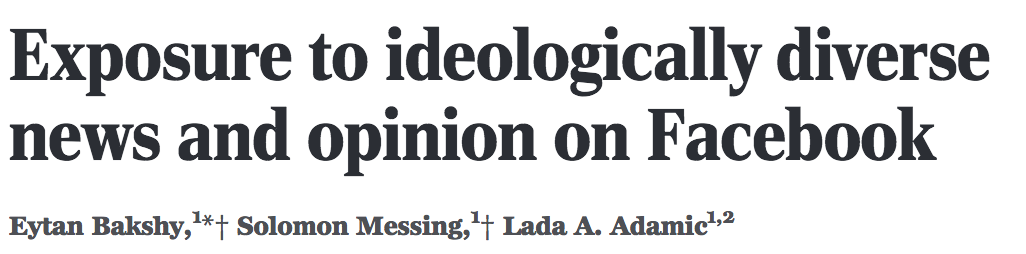
\includegraphics[width=\textwidth]{figures/bakshy_exposure_2015_title}
\end{center}

\note{
focus specifically on the role of algorithms, Facebook NewsFeed
}
\end{frame}
%%%%%%%%%%%%%%%%%%%%
\begin{frame}

\begin{center}
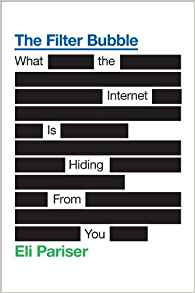
\includegraphics[height=0.95\textheight]{figures/pariser_filter_2011_cover}
\end{center}

\end{frame}
%%%%%%%%%%%%%%%%%%%%%%%%%
\begin{frame}

\begin{center}
\only<1>{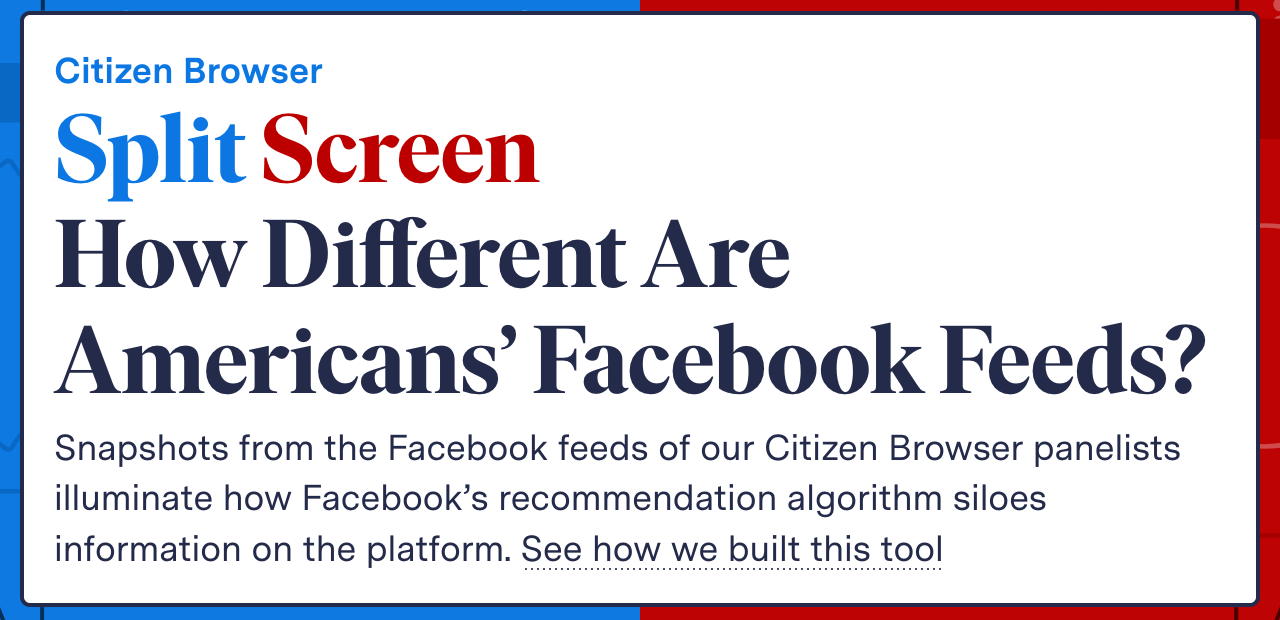
\includegraphics[width=0.95\textwidth]{figures/markup_splitscreen}}%
\only<2->{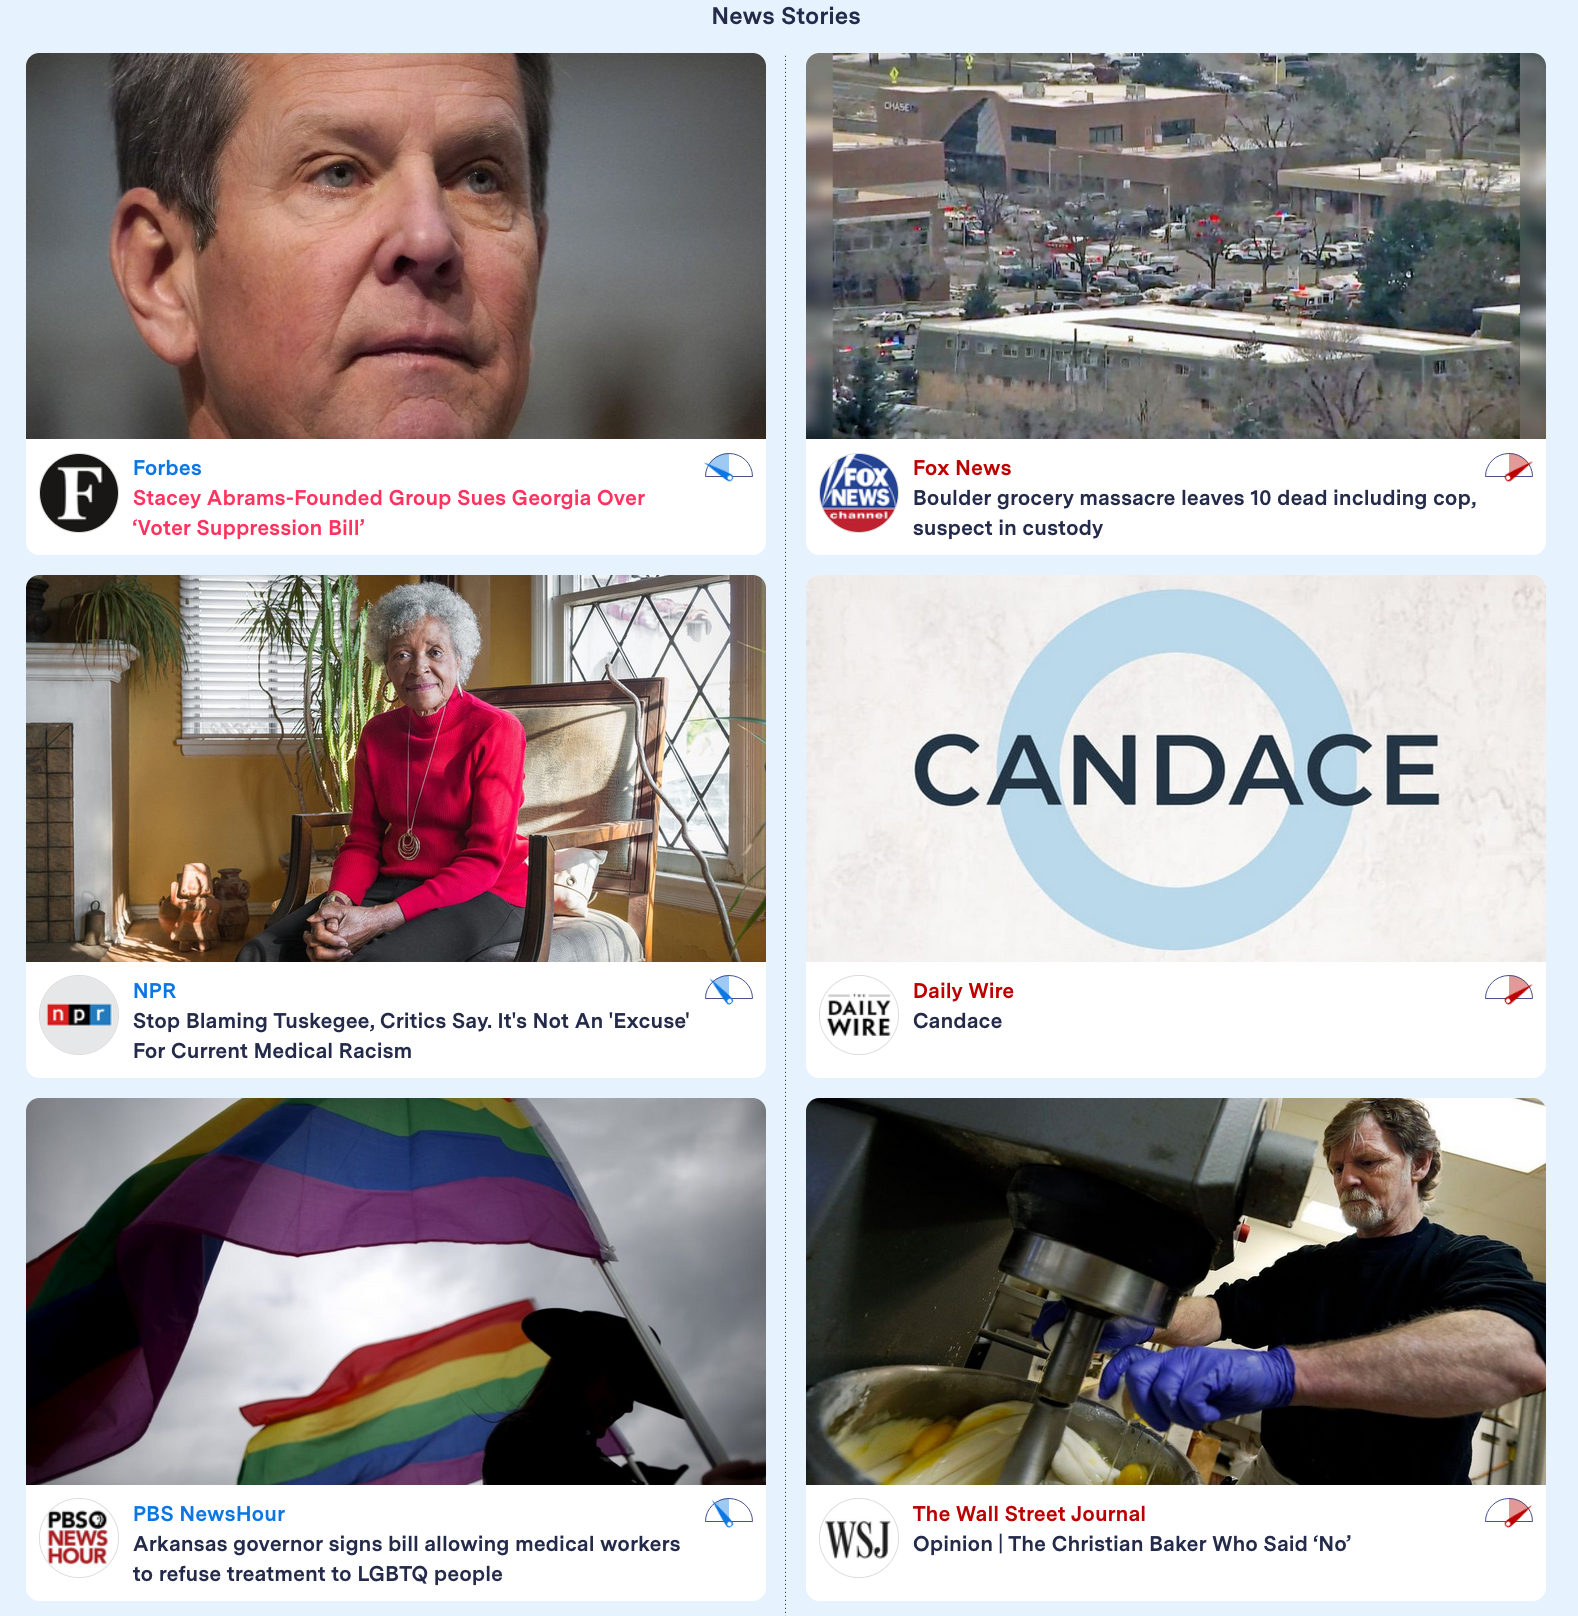
\includegraphics[height=0.85\textheight]{figures/markup_splitscreen_top3}}%
\end{center}

\vfill
\only<2->{Note that these are all political stories, and most stories in NewsFeeds are not political. More info: {\tiny \url{https://themarkup.org/citizen-browser/2021/03/11/introducing-split-screen}}}

\end{frame}
%%%%%%%%%%%%%%%%%%%%%%%%
\begin{frame} 

Information exposure on FB is a multi-step process
\begin{center}
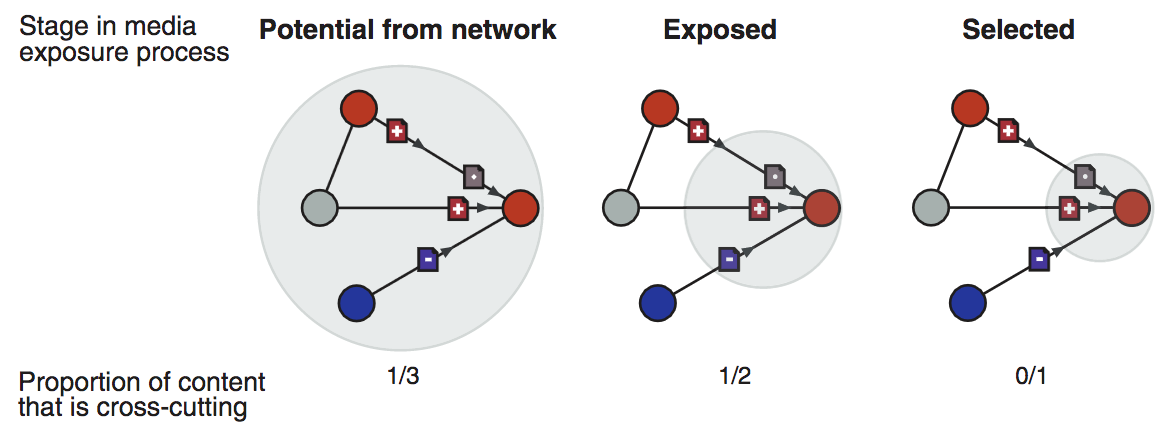
\includegraphics[width=0.95\textwidth]{figures/bakshy_exposure_2015_fig3a}
\end{center}

\end{frame}
%%%%%%%%%%%%%%%%%%%%%%%%%
\begin{frame} 

\begin{center}
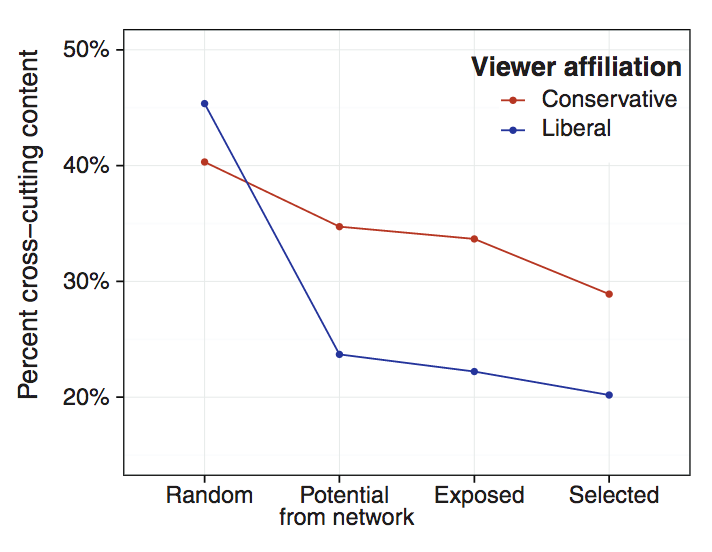
\includegraphics[width=0.8\textwidth]{figures/bakshy_exposure_2015_fig3b}
\end{center}

\end{frame}
%%%%%%%%%%%%%%%%%%%%%%%%%
%\begin{frame} 
%
%Who is included?
%\begin{itemize}
%\item ``we utilize a large, comprehensive dataset from Facebook.''
%\item ``we examined how 10.1 million U.S. Facebook users interact''
%\item in appendix: ``we consider active U.S. adults on Facebook who report their political affiliation.''
%\end{itemize}
%
%\pause
%
%\begin{itemize}
%\item ``18 or older''
%\item ``log in at least 4/7 days per week''
%\item ``have interacted with at least one link shared on Facebook that we classified as hard news''
%\item ``self-report their ideological affiliation in a way that was interpretable''
%\end{itemize}
%
%\vfill
%\pause
%Does this sampling matter?
%
%\end{frame}
%%%%%%%%%%%%%%%%%%%%%%%%%
\begin{frame}

How did they measure the ideology of the subject?
\pause
\begin{center}
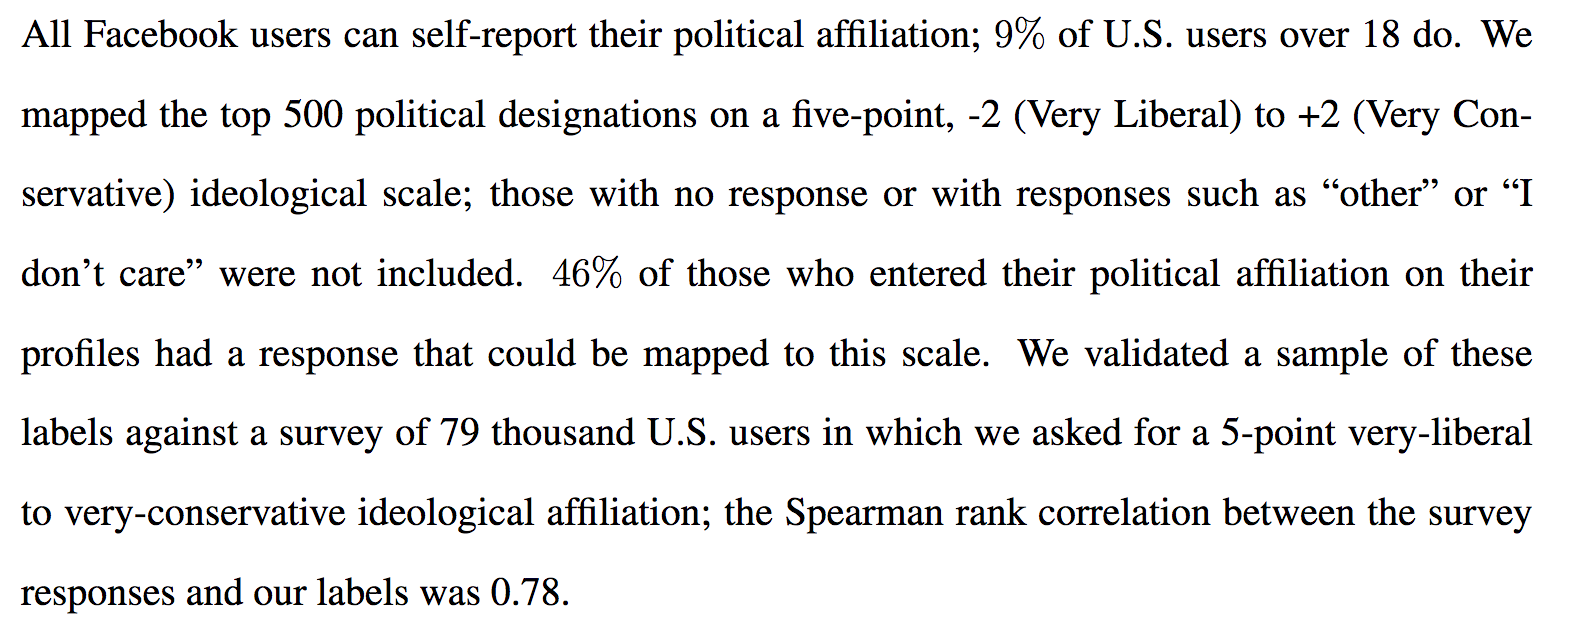
\includegraphics[width=0.95\textwidth]{figures/bakshy_exposure_2015_ego_political}
\end{center}

%\vfill
%\pause
%Does this sampling matter?

\end{frame}
%%%%%%%%%%%%%%%%%%%%%%%%%
\begin{frame}

How did they measure the ideology of the post?
\pause

``We derive the alignment score $A$ of an individual URL by averaging the political alignment of the set of people who share the URL.''

%\vfill
%\pause
%Does this coding scheme matter?

\end{frame}
%%%%%%%%%%%%%%%%%%%%%%%%%
\begin{frame}

What kind of posts?

\pause

``We classified stories as either ``hard'' (such as national news, politics, or world affairs) or ``soft'' content (such as sports, entertainment, or travel) by training a support vector machine on unigram, bigram, and trigram text features (details are available in the supplementary materials, section S1.4.1).''

Approximately 13\% were classified as hard news.  Or approximately 87\% were classified as soft news.  This only counts links shared, not baby pictures.  So we are talking about a small slice of a small slice.

\end{frame}
%%%%%%%%%%%%%%%%%%%%%%%%%
\begin{frame}

\begin{center}
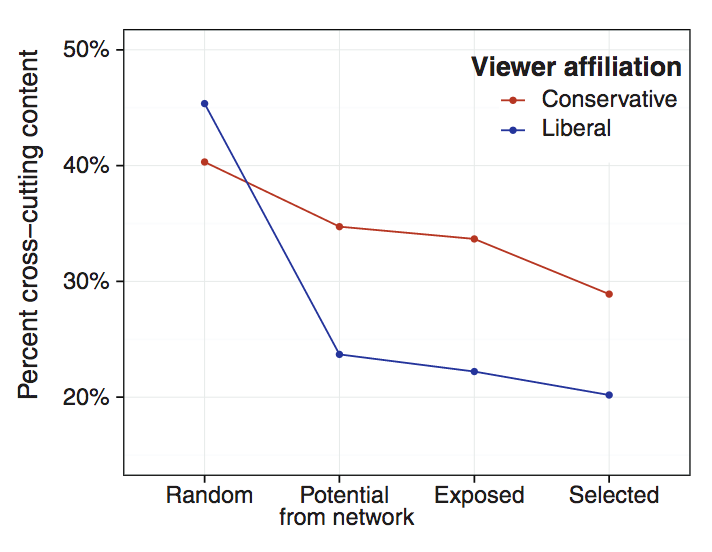
\includegraphics[width=0.8\textwidth]{figures/bakshy_exposure_2015_fig3b}
\end{center}

\end{frame}
%%%%%%%%%%%%%%%%%%%%%%%%%
\begin{frame}

Two interesting, non-filter bubble findings

\end{frame}
%%%%%%%%%%%%%%%%%%%%%%%%%
\begin{frame}

\begin{center}
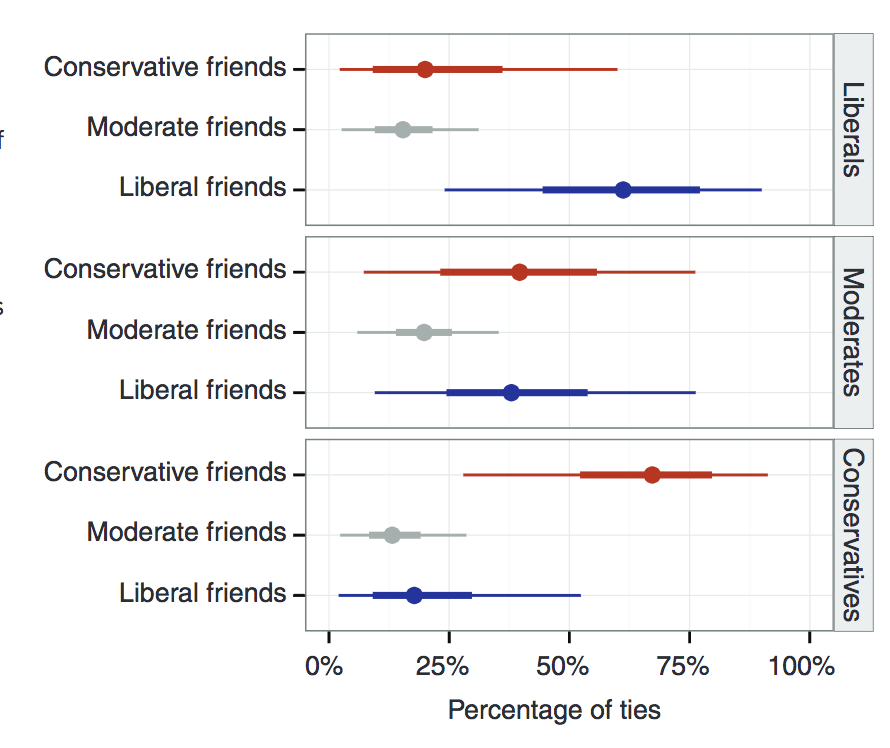
\includegraphics[width=0.70\textwidth]{figures/bakshy_exposure_2015_fig2}
\end{center}

\end{frame}
%%%%%%%%%%%%%%%%%%%%%%%%%
\begin{frame}

\begin{center}
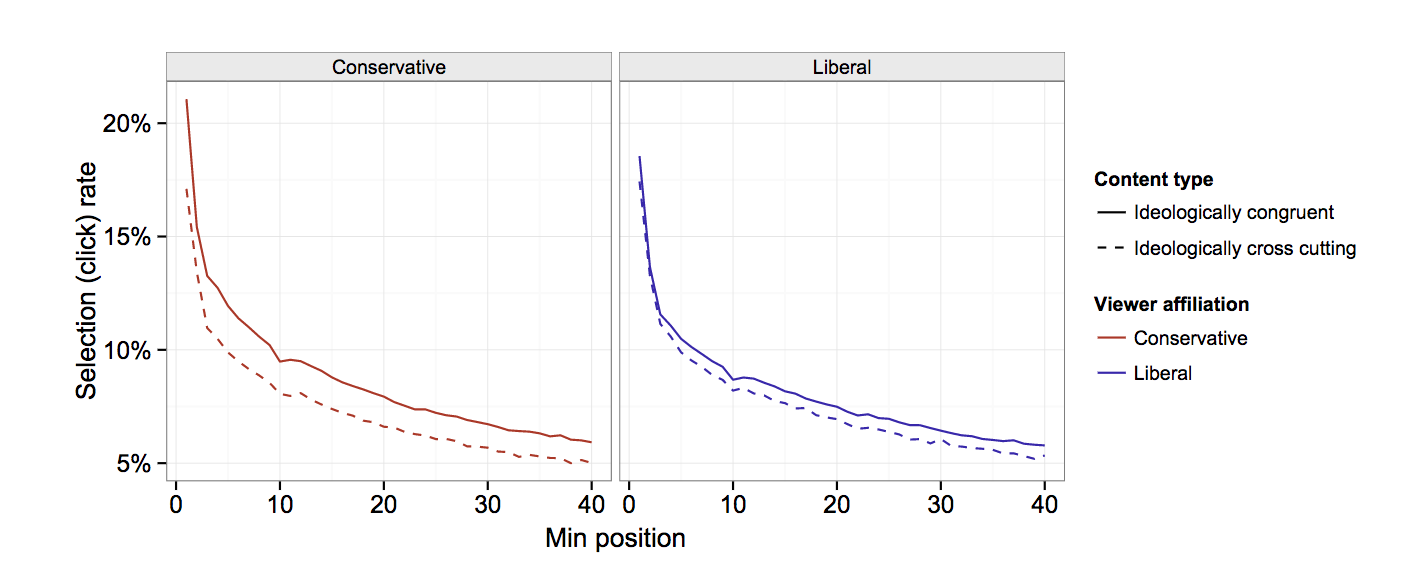
\includegraphics[width=0.8\textwidth]{figures/bakshy_exposure_2015_s5a}
\end{center}

\begin{itemize}
\item people are more likely to click on content at the top of their feed (this might remind you of MusicLab) \pause
\item both liberals and conservatives are more likely to click on ideologically congruent content 
\end{itemize}

\end{frame}
%%%%%%%%%%%%%%%%%%%%%%%%%
\begin{frame}

Is Facebook's NewsFeed algorithm driving political tribalism in the United States? Is it Facebook's fault?
\begin{itemize}
\item ``Compared with algorithmic ranking, individuals' choices played a stronger role in limiting exposure to cross-cutting content.'' \pause
\item ``Within the population under study here, individual choices more than algorithms limit exposure to attitude-challenging content in the context of Facebook.'' \pause
\item ``...our work suggests that the power to expose oneself to perspectives from the other sided in social media lies first and foremost with individuals''
\end{itemize}

\end{frame}
%%%%%%%%%%%%%%%%%%%%%%%%%
\begin{frame}

Commentary and criticism:
\begin{itemize}
\item \url{https://www.wired.com/2015/05/facebook-not-fault-study/}
\item \url{https://medium.com/message/how-facebook-s-algorithm-suppresses-content-diversity-modestly-how-the-newsfeed-rules-the-clicks-b5f8a4bb7bab}
\item \url{https://thesocietypages.org/cyborgology/2015/05/07/facebook-fair-and-balanced/}
\item \url{http://crookedtimber.org/2015/05/07/why-doesnt-science-publish-important-methods-info-prominently/}
\end{itemize}

\end{frame}
%%%%%%%%%%%%%%%%%%%%%%%%%

\begin{frame}

\begin{center}
\Large{Descriptive vs normative}
\end{center}

\note{
What is and what should be
}

\end{frame}
%%%%%%%%%%%%%%%%%%%%%%%%%
\begin{frame}

Thermostat problem:
\begin{itemize}
\item Facebook can control the amount of cross-cutting content that people see.  How should they set the thermostat?
\end{itemize}

\end{frame}
%%%%%%%%%%%%%%%%%%%%%%%%%
\begin{frame}

\begin{center}
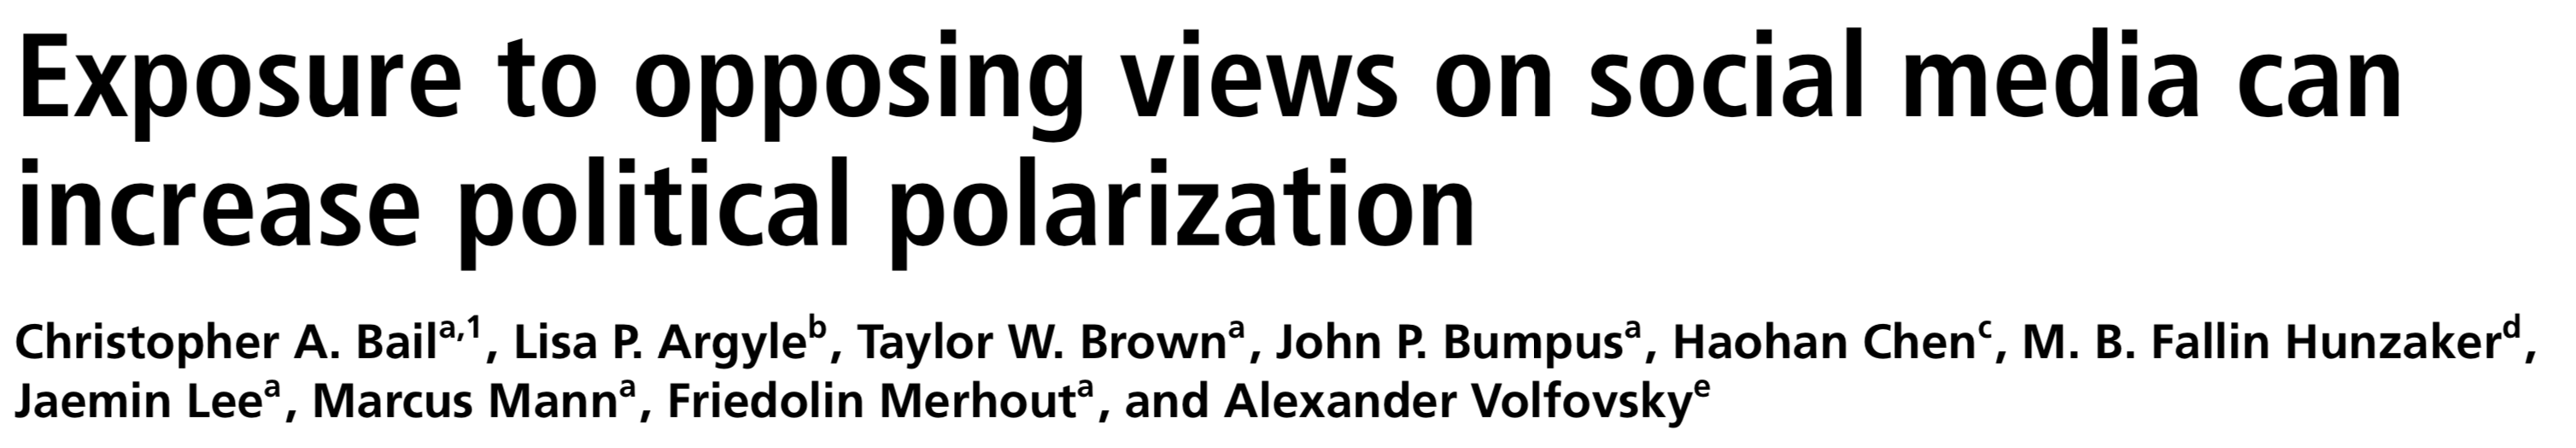
\includegraphics[width=0.80\textwidth]{figures/bail_exposure_2018_title}
\end{center}

\vfill
More cross-cutting content can lead to more polarized attitudes (backfire effect)

\end{frame}
%%%%%%%%%%%%%%%%%%%%%%%%%
\begin{frame}

\begin{itemize}
\item Could someone that didn't work at Facebook do this research? Does that matter? \pause
\item I have received research funding from Facebook, Google, and Microsoft.  Does that matter?  \pause
\item Allcott, Baym, Wagman, and Persaurd all worked at Microsoft Research. Does that matter?
\end{itemize}

\end{frame}
%%%%%%%%%%%%%%%%%%%%%%%%%
\begin{frame}

Are algorithm filter bubbles different from other processes that create filter bubbles? \pause

\begin{center}
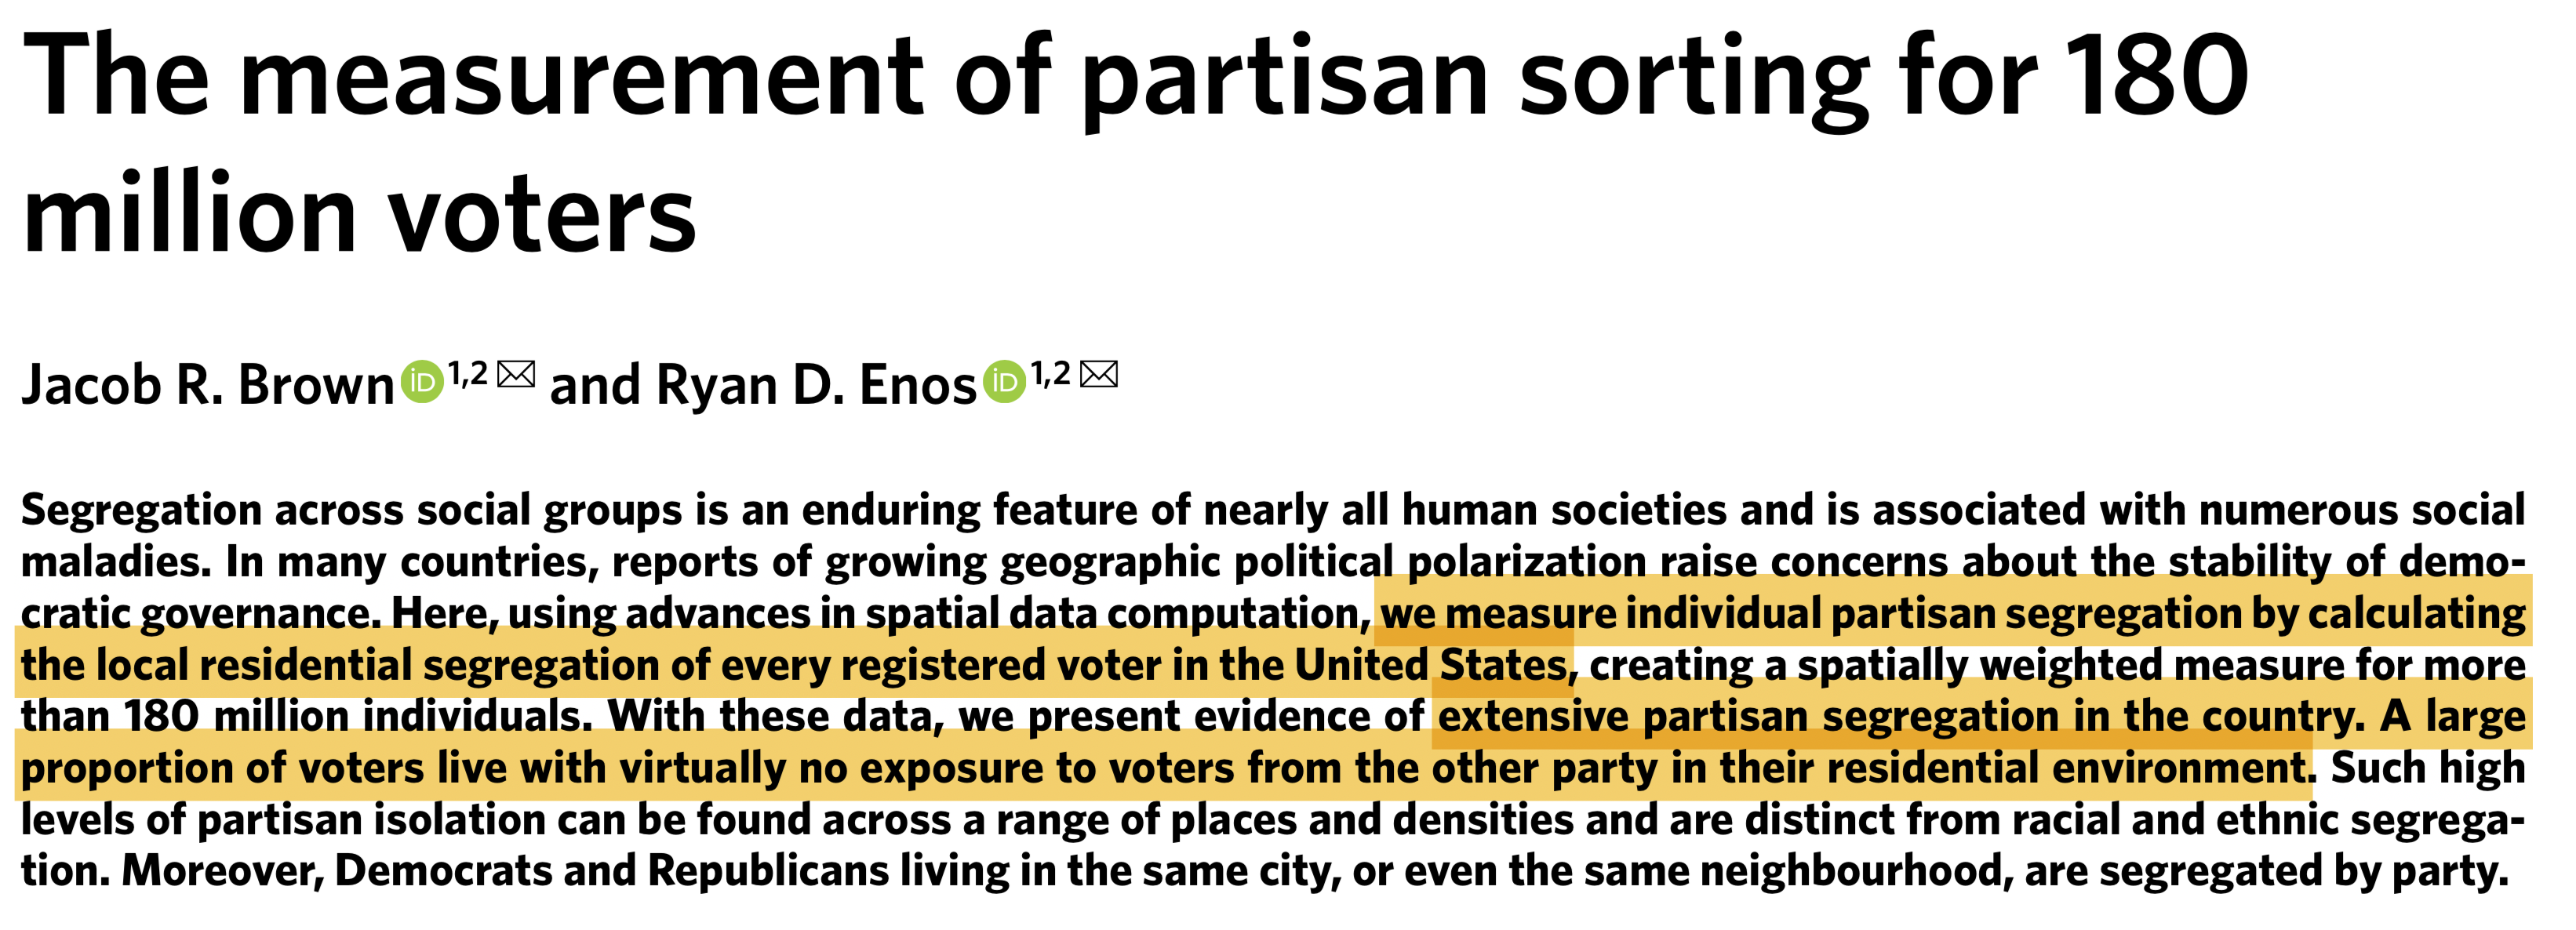
\includegraphics[width=0.80\textwidth]{figures/brown_measurement_2021_titleaabstract}
\end{center}

{\tiny \url{https://www.nytimes.com/interactive/2021/03/17/upshot/partisan-segregation-maps.html}}
\pause

\vfill
I think yes. Algorithmic filter bubbles are centrally controlled and set for profit.

\end{frame}
%%%%%%%%%%%%%%%%%%%%%%%%%
\begin{frame}

\begin{itemize}
\item Social media seems to amplify moral outrage and false rumors \pause
\item This happens because of the choices of people and the choices of social media architects \pause
\item It is hard to isolate how much of this caused by human behavior and how much is magnified by the architecture of the environment
\end{itemize}

\end{frame}
%%%%%%%%%%%%%%%%%%%%%%%%%
\begin{frame}

Center for Information Technology Policy at Princeton works to understand and improve the relationship between technology and society.
\begin{itemize}
\item sign-up for a mailing list: \url{https://citp.princeton.edu/about/contact/subscribe/}
\item learn about undergraduate certificate in Technology and Society, Information Technology Track: \url{https://citp.princeton.edu/programs/certificate/}
\end{itemize}

\end{frame}
%%%%%%%%%%%%%%%%%%%%%%%%%
\begin{frame}

Next class: Social ads in social media
\begin{itemize}
\item Duhigg, C. (2012). How companies learn your secrets. \textit{New York Times}.
\item Goel, S. (2010). Birds of a feather shop together. \textit{Messy Matters blog}.
\item Goel, S. and Goldstein D.G. (2014). Predicting Individual Behavior with Social Networks. \textit{Marketing Science}.
\item Bakshy, E. et al. (2012). Social influence in social advertising: Evidence from field experiments. \textit{EC}
\end{itemize}

\end{frame}
%%%%%%%%%%%%%%%%%%%%%%%%%

\end{document}
